%!TeX program = lualatex
\documentclass[titlepage]{article}
\usepackage{../Head}
\usepackage{relsize}
\graphicspath{.}
\begin{document}
\fancyhf{}
\fancyhead[RO,R]{Advanced Calculus 420}
\fancyhead[LO,L]{Dakota Wicker}
\fancyhead[CO,C]{Homework VIII}
\cfoot{\thepage}

\begin{cproblem}{1}{White}
\ \\
\vspace{-1em}
\begin{center}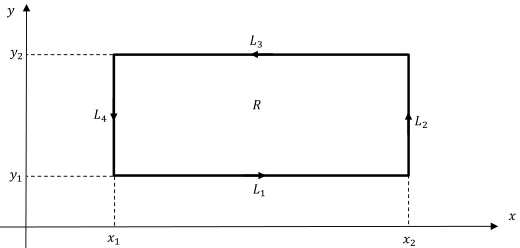
\includegraphics[scale=.75]{rekt.png}\end{center}
It has been shown that given $f(x,y), \ g(x,y), \ \frac{\p f}{\p y},$ and, $\frac{\p g}{\p x}$ are continuous on the rectangle \\
$R = \{(x,y) \ | \ x_1 \leq x \leq x_2, \ y_1 \leq y \leq y_2 \}$, then
$$\bigiint{R}{} \frac{\p g}{\p x} \,dx dy = \mlvarint\limits_{L_2} g \,dy + \mlvarint\limits_{L_4} g \,dy = \mlvarint\limits_{L_2} f \,dx + g \,dy + \mlvarint\limits_{L_4} f \,dx + g \,dy.$$
Apply a similar argument, switching the order of integration in the iterated integral, to obtain
$$\bigiint{R}{}-\frac{\p f}{\p y} \,dx dy = \mlvarint_{L_1} f \,dx + g \,dy \mlvarint_{L_3} f\, dx + g\,dy$$
and complete the proof of Green's Theorem on a rectangle.
\end{cproblem}
\begin{proof}
$$\bigiint{R}{} -\frac{\p f}{\p y} = \mlvarint\limits_{x=x_1}^{x_2} \left[ \mlvarint\limits_{y=y_1}^{y_2} -\frac{\p f}{\p y}\right]dx = \mlvarint\limits_{x_1}^{x^2} f(x,y_2) + f(x,y_1) dx = \mlvarint_{L_1} f(x,y_2) dx + \mlvarint_{L_3} f(x,y_1) dx.$$
Since $dy = 0$, the following is also true
$$\bigiint{R}{} -\frac{\p f}{\p y} = \mlvarint_{L_1} f \,dx + g \,dy + \mlvarint_{L_3} f \,dx + g \,dy.$$
Green's Theorem states that 
$$ \mathlarger\oint_{\p R} f\,dx + g\,dy = \bigiint{R}{}\frac{\p g}{\p x} - \frac{\p f}{ \p y}\,dx dy$$
and by substitution,
\begin{align*}
\mathlarger\oint_{\p R} f \,dx + g \, dy = \bigiint{R}{}\frac{\p g}{\p x} -  \frac{\p f}{ \p y}\,dx dy &= \left[ \mlvarint\limits_{L_2} f \,dx + g \,dy + \mlvarint\limits_{L_4} f \,dx + g \,dy\right] + \left[  \mlvarint_{L_1} f \,dx + g \,dy + \mlvarint_{L_3} f \,dx + g \,dy\right] \\ 
&= \mlvarint\limits_{L_1} f \,dx + g \,dy + \mlvarint\limits_{L_2} f \,dx + g \,dy + \mlvarint_{L_3} f \,dx + g \,dy + \mlvarint_{L_4} f \,dx + g \,dy 
\end{align*}
This proves Green's Theorem for a rectangle.
\end{proof} 

\begin{cproblem}{2}{White}
\ \\
\vspace{-1em}
\begin{itemize}
\item[a.] Prove the following very useful lemma.
\vspace{-1em}
\begin{lemma}{1}\label{sec:1} If $f(x,y)$ is continuous on a region $S$ and $\iint_{R} f\, dx dy = 0$ for every rectangle $R \subset S$, then $f \equiv 0$ on $S$.\end{lemma}
\item[b.] Show that if $f(x,y)$ is such that $\frac{\p f}{\p x}, \ \frac{\p f}{\p y}, \ \frac{\p^2 f}{\p y \p x}, \ \frac{\p^2 f}{\p x \p y}$ are all continuous on a region $S$, then $\frac{\p^2 f}{\p y \p x} = \frac{\p^2 f}{\p x \p y}$ on $S$.
\end{itemize}
\end{cproblem}
\begin{solution}
\vspace{-2em}
\begin{itemize}
\item[a.] \ \\ \vspace{-2em}\begin{proof}\ \\Suppose that $f(x_0, y_0) \neq 0$ for some point $(x_0,y_0) \in S.$ WLOG assume $f(x_0,y_0) > 0$. By continuity there must be a rectangle $R_0 \subset S$ containing $(x_0,y_0)$ where $f(x,y) \geq \frac{f(x_0,y_0)}{2}$ on $R_0.$ This implies that 
$$\bigiint{R}{} f\,dx\,dy \geq \bigiint{R_0}{}f\,dx\,dy \geq x\,y\,\frac{f(x_0,y_0)}{2}$$
and when $\iint_{R_0}f\,dx\,dy = 0$, then
$$\bigiint{R_0}{}f\,dx\,dy = 0 \geq \frac{f(x_0,y_0)}{2}.$$
Since this is clearly not possible because $f(x_0,y_0) > 0$, by contradiction, it must be true that if $\bigiint{R}{}f\,dx\,dy = 0$ for every rectangle $R \subset S$, then $f(x_0,y_0) \equiv 0$ on $S$.
\end{proof}
\item[b.] Green's Theorem on a rectangle states that 
$$  \mathlarger\oint_{\p R} g\,dx + h\,dy = \bigiint{R}{}\frac{\p h}{\p x} - \frac{\p g}{ \p y}\,dx dy $$
for some functions $g(x,y), \ h(x,y)$ where $g, \ h, \ \frac{\p g}{\p y}, \ \frac{\p h}{\p x}$ are all continuous. Let $g = \frac{\p f}{\p y}$ and $h = \frac{\p f}{\p x}$. By Green's Theorem on a rectangle,
$$ \bigiint{R}{}\frac{\p^2 f}{\p x \p y} - \frac{\p^2 f}{ \p y \p x}\,dx dy =  \mathlarger\oint_{\p R} \frac{\p f}{\p x}\,dx + \frac{\p f}{\p y}\,dy.$$
Since $\nabla f = \smat{\frac{\p f}{\p x} \\ \frac{\p f}{\p y}}$ exists, as a result of the fundamental theorem of line integrals $\oint_{\p R} \nabla f \bigcdot d\vec{r} = 0$ so, 
$$ \bigiint{R}{}\frac{\p^2 f}{\p x \p y} - \frac{\p^2 f}{ \p y \p x}\,dx dy =  \mathlarger\oint_{\p R} \frac{\p f}{\p x}\,dx + \frac{\p f}{\p y}\,dy = 0.$$
and by Lemma 1
$$ \bigiint{R}{}\frac{\p^2 f}{\p x \p y} - \frac{\p^2 f}{ \p y \p x}\,dx dy = 0 \implies  \frac{\p^2 f}{\p x \p y} = \frac{\p^2 f}{ \p y \p x}.$$
So, $\frac{\p^2 f}{\p x \p y} = \frac{\p^2 f}{ \p y \p x}$ on $S$.
\end{itemize}
\end{solution}

\begin{cproblem}{3}{White}
Prove Green's Theorem for a general region $S$ in the plane.\\ \\
\textbf{Green's Theorem:} Let $S$ be a region in the plane bounded by the simple closed curve $\p S$ oriented counterclockwise. If $f(x,y), \, g(x,y)$ have continuous partial derivatives on $S \cup \p S$, then
$$\mathlarger\oint_{\p S} f\,dx + g\,dy = \bigiint{S}{}\left(\frac{\p g}{\p x} - \frac{\p f}{\p y}\right)dx\,dy$$
\end{cproblem}
\begin{proof}
I want to prove that
$$\mathlarger\oint_{\p S}f\,dx + g\,dy = \bigiint{S}{}\left(\frac{\p g}{\p x} - \frac{\p f}{\p y} \right) dx\,dy$$
Consider the transformation $x = x(u,v), \ y= y(u,v)$ where the new surface $\p R$ is a rectangle oriented counterclockwise. Then, since we have proven Green's Theorem on a rectangle I will use it here. But first I want to rearrange some elements.
$$\mathlarger\oint_{\p S}f\,dx + g\,dy = \mathlarger\oint_{\p R}(f\,dx + g\,dy) \frac{\p (x,y)}{\p (u,v)}$$
Expanding this I get,
$$ \mathlarger\oint_{\p R}\left(f\,\left(\frac{\p x}{\p u}\,du +\frac{\p x}{\p v}\,dv\right) + g\,\left(\frac{\p y}{\p u}\,du +\frac{\p y}{\p v}\,dv\right)\right) \frac{\p (x,y)}{\p (u,v)}$$
and rearranging these elements in a better order I get
$$\mathlarger\oint_{\p R} \left(\left(f\frac{\p x}{\p u} + g\frac{\p y}{\p u}\right)du + \left(f\frac{\p x}{\p v} + g\frac{\p y}{\p v}\right)dv\right) \frac{\p (x,y)}{\p (u,v)}.$$
Applying Green's Theroem for a rectangle I get,
$$ \mathlarger\oint_{\p R} \left(\left(f\frac{\p x}{\p u} + g\frac{\p y}{\p u}\right)du + \left(f\frac{\p x}{\p v} + g\frac{\p y}{\p v}\right)dv\right) \frac{\p (x,y)}{\p (u,v)} = \bigiint{R}{} \left( \frac{\p \left(f\frac{\p x}{\p v} + g\frac{\p y}{\p v}\right)}{\p u} - \frac{\p \left(f\frac{\p x}{\p u} + g\frac{\p y}{\p u}\right)}{\p v}\right) \frac{\p (x,y)}{\p (u,v)} dudv$$
Doing product rule on these two partial derivatives I get
\begin{align*}
\frac{\p \left(f\frac{\p x}{\p v} + g\frac{\p y}{\p v}\right)}{\p u} &=  \frac{\p f}{\p u}\frac{\p x}{\p v} + f\frac{\p^2 x}{\p u \p v} + \frac{\p g}{\p u} \frac{\p y}{\p v} + g\frac{\p^2 y}{\p u \p v}\\
\frac{\p \left(f\frac{\p x}{\p u} + g\frac{\p y}{\p u}\right)}{\p v} &= \frac{\p f}{\p v}\frac{\p x}{\p u} + f\frac{\p^2 x}{\p v \p u} + \frac{\p g}{\p v} \frac{\p y}{\p u} + g\frac{\p^2 y}{\p v \p u}
\end{align*}
So because $x$ and $y$ are `nice enough',
$$\frac{\p \left(f\frac{\p x}{\p v} + g\frac{\p y}{\p v}\right)}{\p u} -  \frac{\p \left(f\frac{\p x}{\p u} + g\frac{\p y}{\p u}\right)}{\p v}  = \frac{\p f}{\p u}\frac{\p x}{\p v} + \frac{\p g}{\p u} \frac{\p y}{\p v} - \frac{\p f}{\p v}\frac{\p x}{\p u} - \frac{\p g}{\p v} \frac{\p y}{\p u}$$
and rewriting the integral with the jacobian which is
$$\frac{\p(x,y)}{\p(u,v)} = \frac{\p x}{\p u}\frac{\p y}{\p v} - \frac{\p x}{\p v}\frac{\p y}{\p u}$$
I get
$$ \bigiint{R}{}  \left(\frac{\p f}{\p u}\frac{\p x}{\p v} + \frac{\p g}{\p u} \frac{\p y}{\p v} - \frac{\p f}{\p v}\frac{\p x}{\p u} - \frac{\p g}{\p v} \frac{\p y}{\p u}\right)\left( \frac{\p x}{\p u}\frac{\p y}{\p v} - \frac{\p x}{\p v}\frac{\p y}{\p u} \right)du\,dv.$$
Leaving this alone right now, I want to pullback
$$ \bigiint{S}{} \frac{\p g}{\p x} - \frac{\p f}{\p y} dx\,dy.$$
This becomes
$$\bigiint{S}{} \frac{\p g}{\p x} - \frac{\p f}{\p y} dx\,dy = \bigiint{R}{} \left(\frac{\p g}{\p x} - \frac{\p f}{\p y}\right) \frac{\p(x,y)}{\p(u,v)}du\,dv =  \bigiint{R}{} \left(\frac{\p g}{\p x} - \frac{\p f}{\p y}\right) \frac{\p x}{\p u}\frac{\p y}{\p v} - \frac{\p x}{\p v}\frac{\p y}{\p u}du\,dv.$$
Now I want to show that
$$ \bigiint{R}{} \left(\frac{\p g}{\p x} - \frac{\p f}{\p y}\right) \left(\frac{\p x}{\p u}\frac{\p y}{\p v} - \frac{\p x}{\p v}\frac{\p y}{\p u}\right)du\,dv =  \bigiint{R}{}  \left(\frac{\p f}{\p u}\frac{\p x}{\p v} + \frac{\p g}{\p u} \frac{\p y}{\p v} - \frac{\p f}{\p v}\frac{\p x}{\p u} - \frac{\p g}{\p v} \frac{\p y}{\p u}\right)\left( \frac{\p x}{\p u}\frac{\p y}{\p v} - \frac{\p x}{\p v}\frac{\p y}{\p u} \right)du\,dv$$
To do this I expanded the partial derivatives like so
$$\frac{\p f}{\p u}  = \left[\frac{\frac{\p f}{\p x}dx}{du} + \frac{\frac{\p f}{\p y}dy}{du} \right], \ \
\frac{\p f}{\p v}  = \left[\frac{\frac{\p f}{\p x}dx}{dv} + \frac{\frac{\p f}{\p y}dy}{dv}\right], \ \
\frac{\p g}{\p u}  = \left[\frac{\frac{\p g}{\p x}dx}{du} + \frac{\frac{\p g}{\p y}dy}{du}\right] , \ \
\frac{\p g}{\p v}  =\left[\frac{\frac{\p g}{\p x}dx}{dv} + \frac{\frac{\p g}{\p y}dy}{dv}\right] $$
and then through some dense substitution on the R.H.S of this equation and some thick alegbra I get that 
$$\left(\frac{\p f}{\p u}\frac{\p x}{\p v} + \frac{\p g}{\p u} \frac{\p y}{\p v} - \frac{\p f}{\p v}\frac{\p x}{\p u} - \frac{\p g}{\p v} \frac{\p y}{\p u}\right) = \frac{\p g}{\p x} - \frac{\p f}{\p x}.$$
This shows that 
$$ \mathlarger\oint_{\p S}f\,dx + g\,dy = \mathlarger\oint_{\p R}(f\,dx + g\,dy) \frac{\p (x,y)}{\p (u,v)} =  \bigiint{R}{} \left(\frac{\p g}{\p x} - \frac{\p f}{\p y}\right) \left(\frac{\p x}{\p u}\frac{\p y}{\p v} - \frac{\p x}{\p v}\frac{\p y}{\p u}\right)du\,dv = \bigiint{S}{}\left(\frac{\p g}{\p x} - \frac{\p f}{\p y}\right)dx\,dy$$
which proves Green's Theorem.
\end{proof}
\vspace{-.05em}
\begin{cproblem}{4}{White}\ \\
\vspace{-2em}
\begin{center} 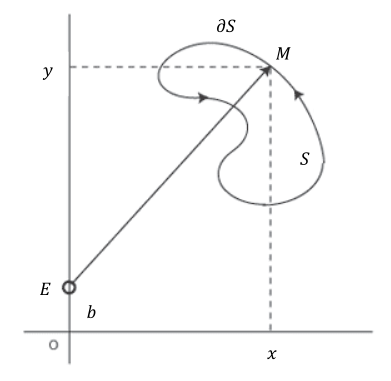
\includegraphics[scale=.45]{planimeter} \end{center}
\begin{itemize}
\vspace{-2em}
\item[a.] Use Green's Theorem to show that
$$ \mathlarger\oint_{\p S} \vec{N} \bigcdot d\vec{X} = \bigiint{S}{}\left( \frac{\p x}{\p x} - \frac{\p (b-y)}{\p y} \right)dx\,dy.$$
\item[b.] Use the fact that $|\vec{N}|$ is constant to show that
$$\frac{\p (b-y)}{\p y} = 0.$$
\item[c.] Conclude that 
$$\mathlarger\oint_{\p S} \vec{N} \bigcdot d\vec{X} = area(S).$$
\end{itemize}
\end{cproblem}
\begin{solution}
\begin{itemize}
\vspace{-2em}
\item[a.] By observing the above diagram, I get that $\vec{EM} = \bmat{x \\ y-b}$. By the relationship of vectors and perpendicular lines, I know that $\vec{N}$ can be described component wise by the negative reciprocal of $\vec{EM}$.
\begin{center}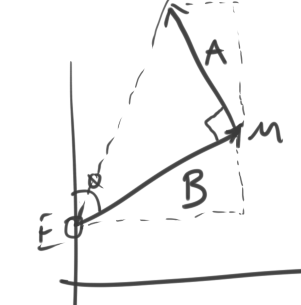
\includegraphics[scale=.6]{perpenslope}\end{center}
As you can see by the diagram, $\Delta A$ is really just a 90 degree  counter clockwise rotation of $\Delta B$. This is always the case when the angle between vectors is 90 degrees. This can be described by taking the negative reciprical componentwise. For example, if I take the negative reciprical componentwise of $\vec{EM} = \smat{x \\ y-b}$ I get $\vec{N} = \smat{-(y-b) \\ x}$ and by rewriting I get $\vec{N} = \smat{b-y \\ x}$. Now, let $f = b-y,  \ g = x$, since all of the conditions of Green's Theorem are met, it is valid to use it. Observe that
$$\mathlarger\oint_{\p S} \bmat{b-y \\ x} \bigcdot \bmat{dx \\ dy} = \mathlarger\oint_{\p S} (b-y)dx + xdy = \mathlarger\oint_{\p S} fdx + gdy$$
and now by applying Green's Theorem I get that
$$ \mathlarger\oint_{\p S} fdx + gdy = \mathlarger\oint_{\p S} (b-y)dx + xdy =    \bigiint{S}{}\left( \frac{\p x}{\p x} - \frac{\p (b-y)}{\p y} \right)dx\,dy.$$
\item[b.] Since $|\vec{N}| = c$ is a constant, it is true that
$$|\vec{N}|^2 = (b-y)^2 + x^2 = c \implies \frac{d (b-y)^2 + x^2}{dy} = 0 \overset{product rule}{\implies} 2(b-y)\left(\frac{d (b-y)}{d y}\right) = 0$$
and when $(b-y) \neq 0$ this implies that $\frac{d (b-y)}{d y} = 0$ and when $(b-y) = 0$, $\frac{d (b-y)}{d y}$ must equal zero, so $\frac{d (b-y)}{d y} = 0$.
\item[c.] Since it is true that $\frac{\p(b-y)}{\p y} = 0$, it is also true that
$$ \mathlarger\oint_{\p S} \vec{N} \bigcdot d\vec{X} = \bigiint{S}{}\left( \frac{\p x}{\p x} - \frac{\p (b-y)}{\p y} \right)dx\,dy = \bigiint{S}{}\,dx\,dy = area(S).$$
\end{itemize}
\end{solution}
\begin{cproblem}{5}{White}
Let $u(x,y,t)$ denote the temperature at point $(x,y)$ of a 2-dimensional plate $P$ at time $t$. Given a rectangle $R\subset P$, the amount of heat energy in $R$ is given by
$$ \bigiint{R}{}c\rho u\,dx\,dy $$
where $c$ is the specific heat of the material and $\rho$ is the mass density of $P$. 
\begin{itemize}
\item[a.] Use the fact that heat flows in the direction of greatest decrease in temperature to show that the `velocity vector' of heat flow is given by
$$ -\kappa\nabla u$$
\item[b.]Show that the flow of heat energy through the boundary of $R$ is given by
$$ \kappa \mathlarger\oint_{\p R} - \frac{\p u}{\p y}dx + \frac{\p u}{\p x}dy$$
\item[c.] Use the fact that
$$ \frac{d}{dt}\left( \bigiint{R}{}c\rho u\,dx\,dy \right) = \kappa \mathlarger\oint_{\p R} - \frac{\p u}{\p y}dx + \frac{\p u}{\p x}dy$$
to show that
$$ c\rho \frac{\p u}{\p t} = \kappa\left(\frac{\p^2 u}{\p x^2} + \frac{\p^2 u}{\p y^2} \right)$$
\end{itemize}
\end{cproblem}
\begin{solution}\ \\
\vspace{-3em}
\begin{itemize}
\item[a.] Since the direction of greatest ascent is the gradient, the greatest descent is going to be the opposite direction. The velocity vector will also grow or shrink by how conductive the material is. So it must be true that the velocity vector of heat will be $-k\nabla u$.
\item[b.] If you notice that
$$ \nabla u = \bmat{\frac{\p u}{\p x} \\ \frac{\p u}{\p y}}, \ d\vec{X} = \bmat{dx \\ dy}$$
and that the velocity vector is
$$ V = -\kappa\nabla u$$
then, by the definition of flux, the total flux is
$$\mathlarger\oint_{\p R} |\bmat{V & d\vec{X}}| = -\kappa \mathlarger\oint_{\p R} \bigg|\bmat{\frac{\p u}{\p x} & dx \\ \frac{\p u}{\p y} & dy}\bigg| = -\kappa \mathlarger\oint_{\p R} - \frac{\p u}{\p y}dx + \frac{\p u}{\p x}dy.$$
\item[c.] Since it is true that
$$\frac{d}{dt}\bigiint{R}{} c\rho u= \kappa \mathlarger\oint_{\p R} -\frac{\p u}{\p y}dx + \frac{\p u}{\p x}dy$$
it is also true that
$$c\rho \bigiint{R}{}\frac{d u}{dt} = \kappa \mathlarger\oint_{\p R} -\frac{\p u}{\p y}dx + \frac{\p u}{\p x}dy$$
and by Green's Theorem,
$$ c\rho \bigiint{R}{}\frac{d u}{dt} = \kappa \bigiint{R}{} \frac{\p^2 u}{\p x^2} + \frac{\p u}{\p y^2}dx\,dy.$$
and by differentiating both sides twice I get
$$\frac{d \left(c\rho \bigiint{R}{}\frac{d u}{dt}\right)}{dx dy} = \frac{d \left(\kappa \bigiint{R}{} \frac{\p^2 u}{\p x^2} + \frac{\p u}{\p y^2}dx\,dy\right)}{dx dy} = c\rho \frac{du}{dt} = \kappa\left(\frac{\p^2 u}{\p x^2} + \frac{\p^2 u}{\p y^2}\right).$$

\end{itemize}
\end{solution}
\end{document}